\section{Проектирование безопасности БД}

\subsection{Основные понятия}

\paragraph{Безопасное программное обеспечение}
Безопасное программное обеспечение - программное обеспечение, разработанное с использованием совокупности
мер, направленных на предотвращение появления и устранение уязвимостей программы \autocite[с. 2]{GOST50939}.

\paragraph{Правила безопасности}
Политика безопасности — это совокупность норм и правил, определяющих принятые в организации меры по
обеспечению безопасности информации, связанной с деятельностью организации. Только человек, четко
осознающий цели организации и условия ее функционирования, может определить, какую информацию
необходимо защищать и насколько существенными могут стать потери от несанкционированного
распространения, искажения или разрушения информации. После того как политика безопасности
определена, должен решаться вопрос о технологии ее реализации в автоматизированном контуре.
Для реализации сформулированных в терминах естественного языка правил и норм политики
безопасности необходимо использовать (или разработать) некоторую формальную модель,
которая допускает эффективное программирование на каком-либо формальном языке.
Наибольшее распространение в настоящее время получили две базовые модели безопасности
данных: дискреционная и мандатная.

\subsection{Методология проектирования}

\subsubsection{Отличия в проектировании безопасных ОС и СУБД}
Системы управления базами данных (СУБД), как и операционные системы, содержат комбинацию сервисов
безопасности, однако, в отличие от ОС, не являются самодостаточными. СУБД используют механизмы
и функции ОС. Такая двухуровневость ведет к появлению специфических угроз и требует привлечения
соответствующих средств противодействия. Например, базы данных располагаются в файлах или на дисках,
управляемых ОС; следовательно, к объектам БД можно обратиться как штатными средствами СУБД, так и с
помощью механизмов ОС, получив доступ к файлу или устройству.
Подобные возможности должны учитываться в профиле защиты для СУБД.
Необходимо реализовать хотя бы один из двух механизмов аутентификации: внешний (аутентификация средствами ОС)
или внутренний (аутентификация средствами СУБД ).
Еще одно проявление упомянутой выше двухуровневости - предположение безопасности базовой конфигурации,
состоящее в том, что базовая система ( операционная система, и/или сетевые сервисы безопасности, и/или
специальное программное обеспечение) установлены, сконфигурированы и управляются безопасным образом.
Аналогичную направленность имеют цели безопасности для среды, предусматривающие, что базовая система
должна обеспечить механизмы управления доступом, которые позволят защитить от несанкционированного доступа
все связанные с СУБД файлы; кроме того, ОС предоставит средства для изоляции функций безопасности и защиты процессов СУБД.
Однако в распределенной информационной системе уровень безопасности может поддерживаться не только средствами базовой ОС,
но и архитектурно, путем разнесения компонентов СУБД по узлам сети и использования межсетевых экранов.

\subsubsection{Основные требования к безопасности СУБД}
Можно выделить меры обеспечения безопасности СУБД зависящие и независящие от данных.
\textbf{Не зависящими} от данных можно назвать следующие требования \autocite{LAPA}:
\begin{itemize}
    \item \textbf{Функционирование в доверенной среде.}
    Под доверенной средой следует понимать инфраструктуру предприятия и ее защитные механизмы,
    обусловленные политиками безопасности. Таким образом, речь идет о функционировании СУБД в
    соответствии с правилами безопасности, применяемыми и ко всем прочим системам предприятия.

    \item \textbf{Организация физической безопасности файлов данных.}
    Требования к физической безопасности файлов данных СУБД в целом не отличаются от требований,
    применяемых к любым другим файлам пользователей и приложений.

    \item \textbf{Организация безопасной и актуальной настройки СУБД.}
    Данное требование включает в себя общие задачи обеспечения безопасности, такие как своевременная
    установка обновлений, отключение неиспользуемых функций или применение эффективной политики паролей.
\end{itemize}
Следующие требования можно назвать \textbf{зависящими} от данных:
\begin{itemize}
    \item \textbf{Безопасность пользовательского ПО.}
    Сюда можно отнести задачи построения безопасных интерфейсов и механизмов доступа к данным.
    \item \textbf{Безопасная организация и работа с данными.}
    Вопрос организации данных и управления ими является ключевым в системах хранения информации.
    В эту область входят задачи организации данных с контролем целостности и другие, специфичные
    для СУБД проблемы безопасности. Фактически эта задача включает в себя основной объем зависящих
    от данных уязвимостей и защиты от них.
\end{itemize}

\subsubsection{Независимые принципы целостности данных}
В работах Кларка и Вильсона определены девять абстрактных теоретических принципов,
выполнение которых позволит обеспечить целостность данных \autocite{Vorobyova}:
\begin{itemize}
    \item \textbf{корректность транзакций;}
    По первому принципу данные могут изменяться только посредством «корректных» транзакций.
    Прямое (произвольным образом) изменение данных не допускается. В свою очередь
    корректность транзакций должна быть некоторым способом доказана.
    \item \textbf{авторизация пользователей;}
    Второй принцип гласит, что изменение данных может осуществляться только
    авторизованными пользователями, имеющими определенные привилегии.
    \item \textbf{минимизация привилегий;}
    Минимальность привилегий подразумевает, что пользователи (в конечном счете, субъекты)
    должны быть наделены теми и только теми привилегиями, которые минимально необходимы
    для выполнения тех или иных действий.
    \item \textbf{разграничение функциональных обязанностей;}
    Разграничение функциональных обязанностей подразумевает организацию работы с данными
    таким образом, что в каждой из ключевых стадий, составляющих единый критически важный
    с точки зрения целостности процесс, необходимо участие различных пользователей.
    Этим гарантируется, что один пользователь не может выполнить весь процесс целиком
    (или даже две его стадии) с тем, чтобы нарушить целостность данных.
    \item \textbf{аудит произошедших событий;}
    Аудит произошедших событий (включая возможность восстановления полной картины происшедшего)
    является превентивной мерой в отношении потенциальных нарушителей и позволяет
    восстановить данные в случае их повреждения.
    \item \textbf{объективный контроль;}
    Принцип объективного контроля также является одним из краеугольных камней политики контроля
    целостности. Суть данного принципа заключается в том, что контроль целостности данных имеет
    смысл лишь тогда, когда эти данные отражают реальное положение вещей. Очевидно, что нет смысла
    заботиться о целостности данных, связанных с размещением боевого арсенала, который уже отправлен
    на переплавку. В связи с этим Кларк и Вильсон указывают на необходимость регулярных проверок,
    целью которых является выявление возможных несоответствий между защищаемыми данными и объективной
    реальностью, которую они отражают.
    \item \textbf{управление передачей привилегий;}
    Управление передачей привилегий необходимо для эффективной работы всей политики безопасности.
    Если схема назначения привилегий неадекватно отражает организационную структуру предприятия или
    не позволяет администраторам безопасности гибко манипулировать ею для обеспечения эффективности
    производственной деятельности, защита становится тяжким бременем и провоцирует попытки обойти ее
    там, где она мешает «нормальной» работе.
    \item \textbf{эффективное применение механизмов защиты;}
    В основу восьмого принципа контроля целостности заложен ряд идей, призванных обеспечить эффективное
    применение имеющихся механизмов обеспечения безопасности. На практике зачастую оказывается, что
    предусмотренные в системе механизмы безопасности или некорректно используются, или полностью
    игнорируются системными администраторами.
    \item \textbf{простота использования защитных механизмов;}
    Простота использования защитных механизмов подразумевает, что самый безопасный путь эксплуатации системы
    будет также наиболее простым, и наоборот, самый простой - наиболее защищенным.
\end{itemize}

\subsubsection{Модель авторизации в System R}
Подход к авторизации в System R основан на списках доступа, с возможностью отмены доступа.
В System R нет администратора базы данных - суперпользователя в обычном смысле. Любой пользователь может создавать таблицы.
Когда пользователь создал таблицу он становится ее суперпользователем.
Если он хочет поделиться своей таблицей с другими пользователями, он может использовать команду GRANT для
предоставления различных привелегий в этой таблице различным пользователям, таким образом составляя
Access List для пользователей, имеющих доступ к таблице, состояющий из UID пользователей.

\subsubsection{Архитектура безопасной СУБД}

Информация взята из \autocite{Rjaibi}

Многоуровневые защищенные архитектуры РСУБД можно разделить на два общих типа, в зависимости от того,
осуществляется ли принудительный контроль доступа самой РСУБД или делегируется доверенной операционной системе.
Эти два основных типа - это архитектура Вудс-Холла и архитектура TrustedSubjects.
\paragraph  {Архитектура Вудс-Холла}
Архитектура Вудс-Холла предполагает, что для доступа к данным используется ненадежная стандартная РСУБД
и что доверенный код разрабатывается вокруг этой РСУБД для обеспечения общей безопасной РСУБД.
Их можно разделить на две категории: ядерные (kernel) архитектуры и распределенные архитектуры.
\paragraph{Ядерная(kernel) архитектура}
Ядерная архитектура использует надежную операционную систему и несколько копий готовой СУБД,
где каждая копия связана с некоторым доверенным интерфейсом. Каждая пара (доверенный интерфейс, СУБД)
связана с определенным уровнем безопасности. Доверенная операционная система применяет свою политику
полного контроля доступа ко всем доступам СУБД к объектам СУБД. Это гарантирует, что данные с разными
уровнями безопасности хранятся отдельно, и что каждая копия СУБД получает доступ к данным, авторизованным
для соответствующего уровня безопасности. Последнее возможно, потому что многоуровневая база данных разбита
на несколько одноуровневых баз данных, каждая из которых представляет собой фрагмент
концептуальной многоуровневой базы данных. Каждый фрагмент хранится в одноуровневом объекте операционной
системы (например, в файле), который помечен операционной системой на соответствующем уровне безопасности,
и, таким образом, к нему можно получить доступ только в соответствии с политикой MAC операционной системы.
\begin{figure}[H]
    \centering
    \includegraphics[width=0.8\textwidth]{assets/security/kernel.png}
    \caption{Ядерная архитектура}
    \label{fig:mesh01}
\end{figure}
На картинке изображена Ядерная архитектура, в которой одна РСУБД связана с уровнем безопасности «Высокий»,
а другая РСУБД связана с уровнем безопасности «Низкий».
РСУБД, связанная с уровнем безопасности «Высокий», имеет доступ как к фрагменту базы данных с высоким уровнем безопасности,
так и к фрагменту базы данных с низким уровнем безопасности. А РСУБД, ассоциированная с уровнем безопасности «Низкий»,
имеет доступ только к фрагменту базы данных с низким уровнем безопасности.
Преимущество этой архитектуры заключается в том, что данные на разных уровнях безопасности изолированы.
Еще одно преимущество состоит в том, что при условии, что надежная операционная система уже готова,
эта архитектура должна минимизировать количество времени и усилий для установки СУБД.
Однако эта архитектура приводит к дополнительным накладным расходам, поскольку доверенной
операционной системе необходимо разделять данные на разных уровнях безопасности при добавлении в базу данных,
а также может потребоваться совершать трудоемкие операции объединения данных с разных уровней безопасности.

\paragraph{Распределенные архитектуры}
Распределенная (или реплицированная) архитектура - это вариант ядерной архитектуры.
Он использует несколько копий доверенного интерфейса и СУБД, каждая из которых связана
со своим собственным хранилищем базы данных. В этой архитектурной схеме СУБД на уровне
безопасности содержит реплику каждого элемента данных, к которому субъект на уровне может получить доступ.
Таким образом, когда данные извлекаются повторно, СУБД извлекает их только из своей собственной базы данных.
Еще одно преимущество этой архитектуры состоит в том, что данные физически разделены на отдельные аппаратные базы данных.
Однако эта схема приводит к дополнительным накладным расходам, когда данные обновляются, поскольку различные
реплики должны быть синхронизированы.
\paragraph{Архитектура TrustedSubjects}
Архитектура TrustedSubjects - это схема, которая содержит надежную СУБД и надежную операционную систему.
Согласно этой архитектуре, политика обязательного контроля доступа обеспечивается самой СУБД.
Объекты базы данных (например, таблица) хранятся в объектах операционной системы (например, в файле) с наивысшим
уровнем безопасности. Таблица базы данных может содержать хранить строки с разными уровнями безопасности.
Такие строки различаются на основе их уровня безопасности, который явно сохраняется с каждой строкой.
Эта архитектура называется TrustedSubjects, потому что РСУБД имеет привилегию нарушать политику MAC
операционной системы при доступе к объектам базы данных. Например, когда пользователь с низким уровнем
безопасности запрашивает таблицу базы данных, к объекту операционной системы, в котором хранится эта таблица,
оказывается, что это является нарушением MAC-политики операционной системы. Но РСУБД способна возвращать пользователям
только те строки, для которых он или она авторизованы в соответствии с политикой MAC.
Преимущество этой архитектуры состоит в том, что СУБД имеет доступ ко всем уровням данных в одно и то же время,
что сводит к минимуму извлечение и обработку обновлений. Однако эта архитектура приводит к созданию специальной
РСУБД, которая требует разработки и проверки большого количества доверенного кода наряду с обычными функциями РСУБД.
Недостатком можно считать недостаточный уровень гарантии аппаратной изоляции объектов.
Также сложно доказать, что доверенное программное обеспечение, используемое для изоляции объектов
(например, потоков данных с разными уровнями безопасности), работает правильно, не допуская потока данных
с высоким уровнем безопасности для пользователей с низким уровнем безопасности.
\begin{figure}[H]
    \centering
    \includegraphics[width=0.8\textwidth]{assets/security/trusted.png}
    \caption{архитектура TrustedSubjects}
    \label{fig:mesh02}
\end{figure}

\subsection{Проектирование безопасных БД}
Разработать универсальную защищенную систему баз данных скорее всего нереально. При любом
разумном методе измерения уровня защищенности этот уровень является неубывающей функцией
от затрат на построение системы защиты. В любом практическом случае, когда существуют
ограничения на бюджет системы защиты, существует и некоторый предельный уровень
информационной безопасности, который теоретически может быть достигнут.

В настоящее время отсутствует общепринятая методология разработки защищенных
автоматизированных информационных систем и, в частности, систем баз данных. В подобных
случаях традиционно используется подход, основанный на анализе лучшего мирового опыта
решения некоторого класса проблем и формулировании руководящих принципов построения
соответствующих систем, концентрирующих накопленный опыт. Именно таким образом для проблемы
обеспечения безопасности информационных систем разрабатывался британский стандарт BS 7799
и созданный на его основе международный стандарт ISO 17799.

Анализ наиболее успешных решений в области обеспечения информационной безопасности баз данных
позволил сформулировать несколько полезных принципов, которыми можно руководствоваться
при проектировании систем защиты:
\begin{itemize}
	\item \textbf{Экономическая оправданность механизмов защиты.}
        Предписывает использование простейшего из всевозможных вариантов проекта, который
        обеспечивает достижение желаемой цели. Хотя этот принцип относится ко многим аспектам
        проектирования систем, он наиболее пригоден при разработке механизмов защиты, так как
        ошибки проектирования и реализации, которые ведут к неконтролируемым способам доступа
        к данным, могут быть не замечены в ходе нормального использования системы. Строгое
        соблюдение этого принципа приводит к применению на практике таких методов, как проверка
        «строка за строкой» программных средств и физическая проверка аппаратных средств,
        реализующих механизмы защиты.

    \item \textbf{Открытое проектирование.}
        Технология систем защиты не должна базироваться на «секретных» алгоритмах. Этот принцип
        широко используется при проектировании безопасных систем и сетей связи. Высокое качество
        систем защиты обеспечивается не недостатком знаний у возможных нарушителей,
        а использованием широко опробованных (как правило, открытых) стандартов и правильной
        организацией управления ключевой информацией. Использование алгоритмов, основанных на
        открытых стандартах в области информационной безопасности, повышает степень доверия
        пользователей к системе защиты и формирует правильную психологическую установку на
        необходимость внимательности и аккуратности при работе с ключевой информацией.

	\item \textbf{Распределение полномочий между различными субъектами в соответствии с правилами организации.}
        Состоит в том, что для критически важных приложений целесообразно использовать многокомпонентные
        схемы доступа к данным. То есть для выполнения соответствующей операции необходимо провести
        аутентификацию нескольких ее обязательных участников. Физический аналог этого принципа можно
        наблюдать в конструкциях банковских сейфов, когда для того, чтобы открыть сейф, необходимо наличие
        двух ключей, которые обычно хранятся у различных людей. Ясно, что механизмы защите, требующие двух
        ключей для доступа к информации, являются более устойчивыми, чем механизмы, которые разрешают доступ
        на основе предъявления единственного ключа. В то же время подобные многокомпонентные процедуры требуют
        больших затрат и, как правило, более сложных процедур управления ключами (включая хранение резервной
        копии). При проектировании многокомпонентных схем доступа за прообраз берется существующая в
        организации практика. Действительно, переход в автоматизированном контуре на более сложные,
        чем использовались «в доавтоматизированную эру», технологии может вызвать психологический дискомфорт
        и различные формы скрытого саботажа системы.

    \item \textbf{Минимально возможные привилегии для пользователей и администраторов.}
        Предписывает, чтобы каждый пользователь (процесс) системы оперировали с данными, используя наименьший
        из возможных набор привилегий, необходимых для выполнения конкретной функции. Применение данного
        принципа нацелено на минимизацию ущерба, который может быть нанесен в случае сбоя, ошибки программного
        обеспечения или компрометации элементов системы защиты данных. Принцип минимальных привилегий,
        используемый при создании пользователей Oracle, — пример реализации этого принципа. Использование
        точек входа SYSTEM и, особенно, SYS должно быть предметом особого регламента. Хорошей практикой
        является использование администратором безопасности нескольких точек входа: обычной, с набором
        привилегий, достаточным для выполнения основных работ, и особой (типа SYSTEM), используемой только
        при возникновении необходимости выполнения действий, требующих высоких привилегий.

    \item \textbf{Управляемость системы при возникновении отказов и сбоев.}
        Проектирование информационной системы, реализованной на базе СУБД, должно осуществляться в предположении,
        что ошибки операционной системы и СУБД, а также сбои аппаратуры неизбежны. При создании системы
        возможность реализации таких событий должна быть учтена: при проектировании процедур и функций должны
        быть обработаны все исключительные ситуации, при обработке данных, содержащих конфиденциальную информацию,
        должны быть минимизированы риски восстановления этих данных по дампам оперативной памяти и содержимому
        временных файлов и т. п. Также должны быть разработаны документы, регламентирующие действия участников
        процесса обработки данных (как пользователей, так и обслуживающего персонала) при возникновении нештатных
        ситуаций. Персонал должен проходить регулярные инструктажи и тренинги по обучению действиям в нештатных
        ситуациях, с иерархией передачи данных.

    \item \textbf{Психологическая приемлемость работы средств защиты данных.}
        Взаимодействие людей с системой (и подсистемой защиты) не должно быть сложным. Пользователи должны
        шаблонно и автоматически применять имеющиеся механизмы защиты. Чрезмерное усложнение механизмов защиты
        может вызывать их внутреннее неприятие и побуждать к использованию различных форм скрытого саботажа.
        Осознанное принятие используемых средств и методов обеспечения информационной безопасности и оценка
        комплекса применяемых мер как необходимых приводит к уменьшению числа ошибок пользователей. В этом случае
        аномальное поведение потенциального нарушителя становится более заметным и проще устанавливается.
        Принцип психологической приемлемости является важным при выборе процедур аутентификации и модели
        управления доступом.
\end{itemize}

\subsubsection{Фазы проектирования безопасных БД (по DoD)}

Министерство обороны (Department of Defence) предложило методологию проектирования, использования и вывода
системы из эксплуатации безопасных информационных систем, в том числе безопасных БД. Стадии жизненного
цикла информационной системы, наиболее часто используемые Министерством обороны, показаны на рис. 6.

\begin{figure}[H]
    \centering
    \includegraphics[width=0.8\textwidth]{assets/security/pic1.png}
    \caption{Стадии жизненного цикла по DoD}
    \label{fig:mesh03}
\end{figure}

Как показано на рис. 6, основная часть жизненного цикла информационной системы включает пять этапов: работа
с требованиями, проектирование архитектуры информационной системы, реализация информационной системы,
тестирование и введение в эксплуатацию. На этапе требований происходит анализ требований заказчика,
формулирование политик безопасности и требований к разрабатываемой информационной системе. На этапе проектирования
архитектуры на основе набора требований, представленного в функциональной форме, составляется концептуальная
модель системы, на основе концептуальной – логическая, на основе логической – физическая.

\subsubsection{Предварительный анализ}

Анализ требований является одним из первых этапов процесса системного проектирования и в некоторой степени
представляет собой интерфейс между внутренними действиями и внешними источниками, предоставляющими входные
данные. В процессе анализа требований исследуются, оцениваются и преобразуются внешние входные данные в
набор функциональных требований, политик безопасности и требований к производительности, которые будут являться
основой для последующего концептуального, логического и физического проектирований. Цель анализа требований –
определение требований к системе.

Анализ миссии системы, анализ среды использования системы определяют потребности клиента и формулируют их в терминах,
которые могут быть использованы для определения функций системы, требований к производительности или проектных
ограничений. Такой анализ определяет функциональные требования к системе, уточняет требования к характеристикам
или проектированию. По мере продвижения этой деятельности исходные предположения и выводы сверяются с меняющимися
деталями. Обычно это приводит к некоторому изменению исходного мышления заказчика, может даже отражаться на его
потребностях, некоторые из которых могут оказаться непрактичными или чрезмерно дорогостоящими.

Результатом анализа требований является набор функциональных определений верхнего уровня и сопутствующих требований
к производительности и архитектуре, которые становятся отправной точкой концептуального проектирования. Анализ
требований проводится итеративно, цикл анализа требований служит для уточнения требований и инициирования
повторной оценки, чтобы определить, насколько жесткими являются требования к элементам системы. Позже подробные
характеристики системы сравниваются с установленными требованиями, чтобы убедиться, что они выполняются.
На этом этапе обычно мало изменений в требованиях из-за обратной связи проверки, но иногда некоторые незначительные
изменения рассматриваются, когда отдача значительна.

\subsubsection{Требования и политики безопасности}

Политика безопасности — это совокупность норм и правил, определяющих принятые в организации меры по обеспечению
безопасности информации, связанной с деятельностью организации. Только человек, четко осознающий цели организации
и условия ее функционирования, может определить, какую информацию необходимо защищать и насколько существенными
могут стать потери от несанкционированного распространения, искажения или разрушения информации. После того как
политика безопасности определена, должен решаться вопрос о технологии ее реализации в автоматизированном контуре.
Для реализации сформулированных в терминах естественного языка правил и норм политики безопасности необходимо
использовать (или разработать) некоторую формальную модель, которая допускает эффективное программирование на
каком-либо формальном языке. Наибольшее распространение в настоящее время получили две базовые модели безопасности
данных: дискреционная и мандатная.

Цель формализации политики безопасности для информационной системы — ясное изложение взглядов руководства
организации на существо угроз информационной безопасности организации и технологий обеспечения безопасности ее
информационных ресурсов. Политика безопасности обычно состоит из двух частей: общих принципов и конкретных правил
работы с информационными ресурсами, то есть требований, и, в частности, с базами данных для различных категорий
пользователей. Политика безопасности – это всегда некоторый компромисс между желаемым уровнем защищенности ресурсов
информационной системы, удобством работы с системой и затратами средств, выделяемых на ее эксплуатацию.

Политика безопасности должна быть оформлена документально на нескольких уровнях управления. На уровне управляющего
высшего звена руководства должен быть подготовлен и утвержден документ, в котором определены цели политики
безопасности, структура и перечень решаемых задач и ответственные за реализацию политики. Основной документ
должен быть детализирован администраторами безопасности информационных систем (управляющими среднего звена)
с учетом принципов деятельности организации, соотношения важности целей, и наличия ресурсов. Детальные решения
должны включать ясные определения методов защиты технических и информационных ресурсов, а также инструкции,
определяющие поведение сотрудников в конкретных ситуациях.

В руководстве по компьютерной безопасности, разработанном национальным институтом стандартов и технологий
США (National Institute of Standards and Technology — NIST), рекомендовано включать в описание
политики безопасности следующие разделы:
\begin{itemize}
	\item \textbf{Предмет политики.}
        В разделе должны быть определены цели и причины разработки политики, область ее применения
        в конкретном фрагменте системы документооборота организации. Должны быть ясно сформулированы
        задачи, решаемые с использованием информационных систем, которые затрагивает данная политика.
        При необходимости могут быть сформулированы термины и определения, используемые в остальных разделах.

    \item \textbf{Описание позиции организации.}
        В этом разделе необходимо ясно описать характер информационных ресурсов организации, перечень
        допущенных к информационным ресурсам лиц и процессов и порядок получения доступа к информационным
        ресурсам организации.

    \item \textbf{Применимость.}
        В разделе может быть уточнен порядок доступа к данным ИС, определены ограничения или технологические
        цепочки, применяемые при реализации политики безопасности.

    \item \textbf{Роли и обязанности.}
        В разделе определяются ответственные должностные лица и их обязанности в отношении разработки и
        внедрения различных элементов политики. Обычно определяются обязанности администратора безопасности
        данных (отвечает за содержательную сторону предоставления доступа к информационным ресурсам организации),
        администратора баз данных (определяет техническую реализацию механизмов разграничения доступа),
        администратора локальной сети, операторов.

    \item \textbf{Соблюдение политики.}
        В разделе описываются права и обязанности пользователей ИС. Необходимо явное описание и документированное
        знакомство пользователей с перечнем недопустимых действий при осуществлении доступа к информационным ресурсам
        организации и наказания за нарушения режимных требований. Должна быть ясно определена технология фиксации
        фактов нарушения политики безопасности и применения административных мер воздействия к нарушителям.
\end{itemize}

Для эффективной реализации политика безопасности должна быть понятной всем пользователям информационных
систем организации. Возможна подготовка презентаций и проведение семинаров с разъяснением основных положений
и практических технологий реализации политики безопасности. Новые сотрудники организации должны быть ознакомлены
или обучены конкретным правилам и технологиям доступа к ресурсам ИС, реализованным в соответствии с принятой
политикой безопасности. Целесообразно проводить контрольные проверки действий сотрудников с обсуждением результатов.

Эффективное проведение политики безопасности возможно только, если она согласована с существующими приказами
и общими задачами организации. Основным способом координации политики безопасности с действующими нормами
организации является ее согласование с заинтересованными подразделениями в ходе разработки.

Комплект документов, представляющий основные решения организации по реализации политики безопасности,
должен включать:
\begin{itemize}
    \item
        документацию, определяющую используемые подходы к оцениванию и управлению рисками для
        организации в целом и при необходимости конкретных подразделений;

    \item
        обоснование принятых решений по выбору средств защиты для рассматриваемой информационной системы;

    \item
        формальное описание процедуры определения допустимого уровня остаточного риска;

    \item
        директиву, определяющую процедуру проверки режима информационной безопасности и журналов,
        в которых фиксируются результаты проверки (документы необходимы для осуществления проверки
        эффективности реализации средств обеспечения информационной безопасности, осуществления
        их контроля качества и правильности использования);

    \item
        документацию, регламентирующую процессы обслуживания и администрирования информационных систем;

    \item
        документацию по подготовке периодических проверок по оцениванию и управлению рисками;

    \item
        документ «Ведомость соответствия», включающий сведения по организации системы управления
        информационной безопасностью и регистрации средств управления безопасностью;

    \item
        контрмеры для противодействия выявленным рискам.
\end{itemize}

Успех проведения в жизнь политики безопасности больше зависит от усилий и опытности людей, реализующих политику,
чем от сложных программно-технических средств контроля.

\subsubsection{Концептуальное проектирование}

Цель этапа концептуального проектирования – создание концептуальной модели данных исходя из представлений
пользователей о предметной области. Для ее достижения выполняется ряд последовательных процедур.
\begin{enumerate}
	\item \textbf{Определение сущностей и их документирование.}
	Для идентификации сущностей определяются объекты, которые существуют независимо от других. Такие объекты
	являются сущностями. Каждой сущности присваивается осмысленное имя, понятное пользователям. Имена и
	описания сущностей заносятся в словарь данных. Если возможно, то устанавливается ожидаемое количество
	экземпляров каждой сущности.
	
	Предположим, что проектируется база данных, предназначенная для хранения информации о деятельности некоторого банка. Этот банк
	имеет филиалы. Филиалы управляются менеджерами. Клиенты имеют в филиалах счета разных типов – текущие, срочные, до востребования, депозитные, карточные.
	Филиалы обрабатывают эти счета. Описываемую предметную область назовем БАНК, в ней могут быть выделены 4 сущности: ФИЛИАЛ, МЕНЕДЖЕР, СЧЕТ, КЛИЕНТ.
	\begin{itemize}
		
		\item ФИЛИАЛ: номер филиала, адрес филиала;
		
		\item МЕНЕДЖЕР: номер менеджера, стаж работы по специальности;
		
		\item СЧЕТ: номер счета, тип счета, дата открытия счета, капитализация (Да/Нет), остаток на счете;
		
		\item КЛИЕНТ: номер клиента, ФИО клиента, адрес клиента, подпись клиента.
		
	\end{itemize}
	
	\item \textbf{Определение связей между сущностями и их документирование.}
	Определяются только те связи между сущностями, которые необходимы для удовлетворения требований к проекту
	базы данных. Устанавливается тип каждой из них. Выявляется класс принадлежности сущностей. Связям
	присваиваются осмысленные имена, выраженные глаголами. Развернутое описание каждой связи с указанием ее
	типа и класса принадлежности сущностей, участвующих в связи, заносится в словарь данных.
	
	В рассматриваемой предметной области БАНК можно выделить 3 связи:
	\begin{itemize}
		
		\item МЕНЕДЖЕР управляет ФИЛИАЛом
		
		\item ФИЛИАЛ обрабатывает СЧЕТ
		
		\item КЛИЕНТ имеет СЧЕТ
		
	\end{itemize}
	
	\item \textbf{Создание ER-модели предметной области.}
	Для представления сущностей и связей между ними используются ER-диаграммы. На их основе создается единый
	наглядный образ моделируемой предметной области – ER-модель предметной области.
	
	На диаграмме сущность изображается прямоугольником, в
	котором указывается ее имя. А связь ромбом. Так же важен тип связи(1:1, 1:M, M:N). Рассмотрим их подробнее:
	\begin{itemize}
		\item 1:1(один к одному): примером такой связи служит "МЕНЕДЖЕР управляет ФИЛИАЛом", так как МЕНЕДЖЕР управляет только одним ФИЛИАЛом, а ФИЛИАЛ имеет только одного МЕНЕДЖЕРа;
		
		\item 1:M(один ко многим): примером такой связи служит "ФИЛИАЛ  обрабатывает СЧЕТ", так как СЧЕТ обрабатывается только одним ФИЛИАЛом, а ФИЛИАЛ может обрабатывать более одного СЧЕТа;
		
		\item  M:N(многие ко многим): примером такой связи служит "КЛИЕНТ ИМЕЕТ СЧЕТ", так как СЧЕТ может быть совместным и им могут пользоваться сразу несколько КЛИЕНТов, а КЛИЕНТ может завести более одного СЧЕТа;
	\end{itemize}
	\begin{figure}[H]
		\centering
		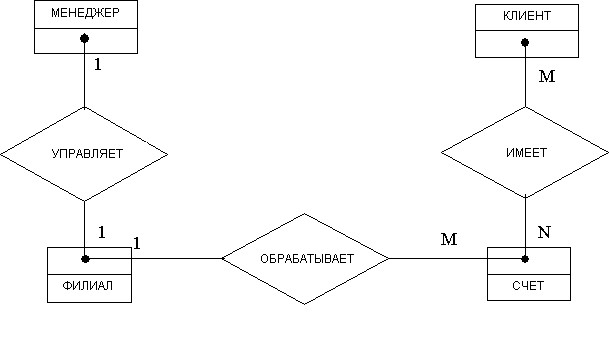
\includegraphics[width=0.8\textwidth]{assets/security/pic25.png}
		\caption{ER-модель предметной области БАНК}
		\label{fig:mesh28}
	\end{figure}
	
	\item \textbf{Определение атрибутов и их документирование.}
	Выявляются все атрибуты, описывающие сущности созданной ER-модели. Каждому атрибуту присваивается осмысленное
	имя, понятное пользователям. О каждом атрибуте в словарь данных помещаются следующие сведения:
	\begin{itemize}
		\item имя атрибута и его описание;
		
		\item тип и размерность значений;
		
		\item значение, принимаемое для атрибута по умолчанию (если такое имеется);
		
		\item может ли атрибут иметь NULL-значения;
		
		\item является ли атрибут составным, и если это так, то из каких простых атрибутов он состоит.
		Например, атрибут "Ф.И.О. клиента" может состоять из простых атрибутов "Фамилия", "Имя",
		"Отчество", а может быть простым, содержащим единые значения, как-то "Сидорский Евгений
		Михайлович". Если пользователь не нуждается в доступе к отдельным элементам "Ф.И.О.",
		то атрибут представляется как простой;
		
		\item является ли атрибут расчетным, и если это так, то как вычисляются его значения.
	\end{itemize}
	
	\item \textbf{Определение значений атрибутов и их документирование.}
	Для каждого атрибута сущности, участвующей в ER-модели, определяется набор допустимых значений и ему
	присваивается имя. Например, атрибут "Тип счета" может иметь только значения "депозитный", "текущий",
	"до востребования", "карт-счет". Обновляются записи словаря данных, относящиеся к атрибутам, – в них
	заносятся имена наборов значений атрибутов.
	
	\item \textbf{Определение первичных ключей для сущностей и их документирование.}
	На этом шаге руководствуются определением первичного ключа – как атрибута или набора атрибутов сущности,
	позволяющего уникальным образом идентифицировать ее экземпляры. Сведения о первичных ключах помещаются
	в словарь данных.
	
	\item \textbf{Обсуждение концептуальной модели данных с конечными пользователями.}
	Концептуальная модель данных представляется ER-моделью с сопроводительной документацией, содержащей
	описание разработанной модели данных. Если будут обнаружены несоответствия предметной области, то в
	модель вносятся изменения  до тех пор, пока пользователи не подтвердят, что предложенная им модель
	адекватно отображает их личные представления.
\end{enumerate}

\subsubsection{Логическое  проектирование}

Цель этапа логического проектирования – преобразование концептуальной модели на основе выбранной модели данных
в логическую модель, не зависимую от особенностей используемой в дальнейшем СУБД для физической реализации базы
данных. Для ее достижения выполняются следующие процедуры:
\begin{enumerate}
    \item \textbf{Выбор модели данных.}
        Чаще всего выбирается реляционная модель данных в связи с наглядностью табличного представления данных
        и удобства работы с ними.

    \item \textbf{Определение набора таблиц исходя из ER-модели и их документирование.}
        Для каждой сущности ER-модели создается таблица. Имя сущности – имя таблицы. Причем каждому атрибуту
        сущности соответствует столбец таблицы. Правила генерации таблиц из ER-диаграмм опираются на два основных
        фактора – тип связи и класс принадлежности сущности. Устанавливаются связи между таблицами посредством
        механизма первичных и внешних ключей. Структуры таблиц и установленные связи между ними документируются.

        Изложим правила генерации таблиц из ER-диаграмм, используя пример ER-модели предметной
        области БАНК, представленной на рис. 7, со следующими наборами атрибутов сущностей предметной области БАНК,
        представленными на рис. 8.

    \begin{figure}[H]
        \centering
        \includegraphics[width=0.8\textwidth]{assets/security/pic2.png}
        \caption{Пример ER-модели предметной области БАНК}
        \label{fig:mesh04}
    \end{figure}

    \begin{figure}[H]
        \centering
        \includegraphics[width=0.8\textwidth]{assets/security/pic3.png}
        \caption{Наборы атрибутов сущностей предметной области БАНК}
        \label{fig:mesh05}
    \end{figure}

    Для связи типа 1:1 существуют три отдельных правила формирования предварительных таблиц из ER-диаграмм.

    \underline{Правило 1}

    Если связь типа 1:1 и класс принадлежности обеих сущностей является обязательным, то необходима только одна
    таблица. Первичным ключом этой таблицы может быть первичный ключ любой из двух сущностей.

    На ER-диаграмме связи 1:1, класс принадлежности сущностей МЕНЕДЖЕР, ФИЛИАЛ является обязательным. Тогда согласно
    правилу 1 должна быть сгенерирована одна таблица следующей структуры:

    \begin{figure}[H]
        \centering
        \includegraphics[width=100mm]{assets/security/pic4.png}
        \label{fig:mesh06}
    \end{figure}

    Первичным ключом этой таблицы может быть и первичный ключ сущности МЕНЕДЖЕР – НМ.

    \underline{Правило 2}

    Если связь типа 1:1 и класс принадлежности одной сущности является обязательным, а другой – необязательным,
    то необходимо построить таблицу для каждой сущности. Первичный ключ сущности должен быть первичным ключом
    соответствующей таблицы. Первичный ключ сущности, для которой класс принадлежности является необязательным,
    добавляется как атрибут в таблицу для сущности с обязательным классом принадлежности.

    Представим, что на ER-диаграмме связи 1:1, изображенной на рис. 7, класс принадлежности сущности МЕНЕДЖЕР
    будет обязательный, а сущности ФИЛИАЛ – необязательный. Тогда согласно правилу 2 должны быть сгенерированы
    две таблицы следующей структуры:

    \begin{figure}[H]
        \centering
        \includegraphics[width=100mm]{assets/security/pic5.png}
        \label{fig:mesh07}
    \end{figure}

    Сущность с необязательным классом принадлежности (ФИЛИАЛ) именуется родительской, а с обязательным (МЕНЕДЖЕР)
    – дочерней. Первичный ключ родительской сущности (НФ), помещаемый в таблицу, представляющую дочернюю сущность,
    называется внешним ключом родительской сущности. Связь между указанными таблицами устанавливается путем связи
    первичного и внешнего ключа и имеет вид:

    \begin{figure}[H]
        \centering
        \includegraphics[width=0.8\textwidth]{assets/security/pic6.png}
        \label{fig:mesh08}
    \end{figure}

    Примечание. Если внешний ключ представляет связь 1:1, то должны быть запрещены его дублирующие значения.

    \underline{Правило 3}

    Если связь типа 1:1 и класс принадлежности обеих сущностей является необязательным, то необходимо построить
    три таблицы – по одной для каждой сущности и одну для связи. Первичный ключ сущности должен быть первичным
    ключом соответствующей таблицы. Таблица для связи среди своих атрибутов должна иметь ключи обеих сущностей.

    Представим, что на ER-диаграмме связи 1:1, изображенной на рис. 7, класс принадлежности сущностей МЕНЕДЖЕР,
    ФИЛИАЛ будет необязательный. Тогда согласно правилу 3 должны быть сгенерированы три таблицы следующей структуры:

    \begin{figure}[H]
        \centering
        \includegraphics[width=100mm]{assets/security/pic7.png}
        \label{fig:mesh09}
    \end{figure}

    При этом осуществляется декомпозиция связи 1:1 на две связи 1:1 следующим образом:

    \begin{figure}[H]
        \centering
        \includegraphics[width=0.8\textwidth]{assets/security/pic8.png}
        \label{fig:mesh10}
    \end{figure}

    Для связи типа 1:М существуют только два правила. Выбор одного из них зависит от класса принадлежности
    сущности на стороне M. Класс принадлежности сущности на стороне 1 не влияет на выбор.

    \underline{Правило 4}

    Если связь типа 1:М и класс принадлежности сущности на стороне М является обязательным, то необходимо
    построить таблицу для каждой сущности. Первичный ключ сущности должен быть первичным ключом соответствующей
    таблицы. Первичный ключ сущности на стороне 1 добавляется как атрибут в таблицу для сущности на стороне М.

    На ER-диаграмме связи 1:М, представленной на рис. 7, класс принадлежности сущности СЧЕТ является обязательным.
    Тогда согласно правилу 4 должны быть сгенерированы две таблицы следующей структуры:

    \begin{figure}[H]
        \centering
        \includegraphics[width=100mm]{assets/security/pic9.png}
        \label{fig:mesh11}
    \end{figure}

    Связь между указанными таблицами будет иметь вид:

    \begin{figure}[H]
        \centering
        \includegraphics[width=0.8\textwidth]{assets/security/pic10.png}
        \label{fig:mesh12}
    \end{figure}

    Примечание. Если внешний ключ представляет связь 1:М, то должны быть разрешены его дублирующие значения.

    \underline{Правило 5}

    Если связь типа 1:М и класс принадлежности сущности на стороне М является необязательным,
    то необходимо построить три таблицы – по одной для каждой сущности и одну для связи. Первичный ключ сущности
    должен быть первичным ключом соответствующей таблицы. Таблица для связи среди своих атрибутов должна
    иметь ключи обеих сущностей.

    Представим, что на ER-диаграмме связи 1:М, изображенной на рис. 7, класс принадлежности сущности СЧЕТ
    является необязательным. Тогда согласно правилу 5 должны быть сгенерированы три таблицы следующей структуры:

    \begin{figure}[H]
        \centering
        \includegraphics[width=100mm]{assets/security/pic11.png}
        \label{fig:mesh13}
    \end{figure}

    При этом осуществляется декомпозиция связи 1:М на две связи – 1:М и 1:1 – следующим образом

    \begin{figure}[H]
        \centering
        \includegraphics[width=0.8\textwidth]{assets/security/pic12.png}
        \label{fig:mesh14}
    \end{figure}

    Для связи типа М:N класс принадлежности сущности не имеет значения.

    \underline{Правило 6}

    Если связь типа М:N, то необходимо построить три таблицы – по одной для каждой сущности и одну для связи.
    Первичный ключ сущности должен быть первичным ключом соответствующей таблицы. Таблица для связи среди своих
    атрибутов должна иметь ключи обеих сущностей.

    ER-диаграмма связи М:N имеется на рис. 7. Согласно правилу 6 на основе этой ER-диаграммы должны быть
    сгенерированы три таблицы следующей структуры:

    \begin{figure}[H]
        \centering
        \includegraphics[width=100mm]{assets/security/pic13.png}
        \label{fig:mesh15}
    \end{figure}

    При этом осуществляется декомпозиция связи М:N на две связи 1:М следующим образом:

    \begin{figure}[H]
        \centering
        \includegraphics[width=0.8\textwidth]{assets/security/pic14.png}
        \label{fig:mesh16}
    \end{figure}

    В таблице КЛИЕНТ–СЧЕТ клиенту, имеющему, например, три счета будут соответствовать три строки
    с одним и тем же номером клиента. А счет, у которого, например, два владельца, представляется двумя
    строками с различными номерами клиентов, владеющими этим счетом.

    К ER-модели предметной области БАНК, представленной на рис. 7, применимы правила 1, 4, 6. Связь МЕНЕДЖЕР
    – ФИЛИАЛ представляется (согласно правилу 1) одной таблицей А:

    \begin{figure}[H]
        \centering
        \includegraphics[width=0.8\textwidth]{assets/security/pic15.png}
        \label{fig:mesh17}
    \end{figure}

    Связь ФИЛИАЛ – СЧЕТ  представляется (согласно правилу 4) связью:

    \begin{figure}[H]
        \centering
        \includegraphics[width=0.8\textwidth]{assets/security/pic16.png}
        \label{fig:mesh18}
    \end{figure}

    Связь КЛИЕНТ – СЧЕТ представляется (согласно правилу 6) связью:

    \begin{figure}[H]
        \centering
        \includegraphics[width=0.8\textwidth]{assets/security/pic17.png}
        \label{fig:mesh19}
    \end{figure}

    Анализ состава атрибутов полученных таблиц A, B, C, D, E, F показывает, что таблица В является составной
    частью таблицы А, таблица Е – составной частью таблицы С. Поэтому таблицы В, Е можно исключить из рассмотрения.
    Оставшиеся таблицы А, С, D, F можно связать посредством связи первичных и внешних ключей.
    В результате получим реляционную модель для ER-модели предметной области БАНК.

    \item \textbf{Нормализация таблиц.}
        Для правильного выполнения нормализации проектировщик должен глубоко изучить семантику и особенности
        использования данных. На этом шаге он проверяет корректность структуры таблиц, созданных на предыдущем
        шаге, посредством применения к ним процедуры нормализации. Она заключается в приведении каждой из таблиц,
        по крайней мере, к 3НФ. В результате нормализации получается очень гибкий проект базы данных,
        позволяющий легко вносить в нее нужные расширения.

        Нормализация таблиц - процесс, позволяющий минимизировать избыточность данных. Чтобы пояснить этот процесс,
        будем исходить из описания предметной области БАНК, представленного на рис. 7, и предположения, что на его
        основе была разработана база данных, состоящая из следующих двух таблиц:

    \begin{figure}[H]
        \centering
        \includegraphics[width=0.8\textwidth]{assets/security/pic18.png}
        \label{fig:mesh20}
    \end{figure}

    \underline{1 нормальная форма (1НФ)}

    Таблица находится в 1НФ, если все ее поля содержат только простые неделимые значения.

    Таблицы ФИЛИАЛ и КЛИЕНТ не удовлетворяют требованиям 1НФ. Для приведения их к 1НФ в них надо вставить новые
    записи следующим образом:

    \begin{figure}[H]
        \centering
        \includegraphics[width=0.8\textwidth]{assets/security/pic19.png}
        \label{fig:mesh21}
    \end{figure}

    Но полученные таблицы неэффективны, так как содержат много избыточной информации. Необходимо их привести к 2НФ.

    \underline{2 нормальная форма (2НФ)}

    Таблица находится в 2НФ, если она удовлетворяет требованиям 1НФ и неключевые поля функционально полно
    зависят от первичного ключа.

    Функциональная зависимость – это понятие, отображающее определенную семантическую связь между полями таблицы.
    Неключевое поле А функционально полно зависит от первичного ключа, если:
    \begin{enumerate}
        \item оно функционально зависит от первичного ключа, т.е. каждой комбинации значений полей первичного
        ключа соответствует одно и только одно значение поля А;

        \item не существует функциональной зависимости А ни от какого подмножества полей первичного ключа
        (в противном случае А находится в частичной функциональной зависимости от первичного ключа).
    \end{enumerate}

    В таблице КЛИЕНТ неключевые поля ФИО\_К, СОЦ\_П, АДР\_К функционально зависят от ключа (НК, НС). Кроме того,
    они функционально зависят от подмножества ключа – НК. Следовательно, неключевые поля ФИО\_К, СОЦ\_П, АДР\_К
    находятся в частичной функциональной зависимости от первичного ключа (НК, НС) и нарушаются требования 2НФ.
    Эти поля надо из таблицы КЛИЕНТ удалить. Полученную в результате этого таблицу назовем КЛИЕНТ–СЧЕТ, которая
    имеет вид:

    \begin{figure}[H]
        \centering
        \includegraphics[width=40mm]{assets/security/pic20.png}
        \label{fig:mesh22}
    \end{figure}

    Эта таблица удовлетворяет требованиям 2НФ.

    Удаленные неключевые поля помещаются в новую таблицу совместно с подмножеством НК, от которого они зависят.
    И это подмножество будет первичным ключом новой таблицы КЛИЕНТ вида:

    \begin{figure}[H]
        \centering
        \includegraphics[width=0.8\textwidth]{assets/security/pic21.png}
        \label{fig:mesh23}
    \end{figure}

    Новая таблица КЛИЕНТ также удовлетворяет требованиям 2НФ. Ее неключевые поля функционально полно зависят
    от первичного ключа.

    Полученные таблицы не содержат избыточной информации, и нет основания приводить их к 3НФ. Таблица ФИЛИАЛ
    удовлетворяет требованиям 2НФ, так как ее неключевые поля НФ, АДР\_Ф, НМ, ОСТ, ТИП функционально полно
    зависят от первичного ключа. Но в таблице ФИЛИАЛ повторяется информация о филиале для всех счетов,
    обрабатываемых им. Поэтому ее надо привести к 3НФ.

    \underline{3 нормальная форма (3НФ)}

    Таблица находится в 3НФ, если она удовлетворяет требованиям 2НФ и не содержит транзитивных зависимостей.

    Транзитивной зависимостью называется функциональная зависимость между неключевыми полями. В таблице ФИЛИАЛ
    она наблюдается. Следовательно, нарушаются требования 3НФ. Из таблицы ФИЛИАЛ надо удалить поля, участвующие
    в этой транзитивной зависимости, – АДР\_Ф, НМ. Получится таблица, характеризующая счет, вида:

    \begin{figure}[H]
        \centering
        \includegraphics[width=100mm]{assets/security/pic22.png}
        \label{fig:mesh24}
    \end{figure}

    Затем создается новая таблица, в которую помещаются удаленные поля и поле, от которого они зависят. Она имеет вид:

    \begin{figure}[H]
        \centering
        \includegraphics[width=100mm]{assets/security/pic23.png}
        \label{fig:mesh25}
    \end{figure}

    Полученные таблицы приведены к 3НФ. В них каждая запись есть отдельное независимое утверждение. Повторяются
    только значения внешнего ключа НФ в таблице СЧЕТ, что неизбежно, так как одним филиалом могут обрабатываться
    несколько счетов.

    Как видим, нормализация приводит к фрагментации исходных таблиц. В нашем примере таблица КЛИЕНТ разбивается
    на таблицы 1, 2, а таблица ФИЛИАЛ  – на таблицы 3, 4. Осуществив связь этих таблиц посредством связи первичных
    и внешних ключей, получим реляционную модель данных предметной области БАНК, в которой минимизирована
    избыточность данных:

    \begin{figure}[H]
        \centering
        \includegraphics[width=0.8\textwidth]{assets/security/pic24.png}
        \label{fig:mesh26}
    \end{figure}

    \item \textbf{Проверка логической модели данных на предмет возможности выполнения всех транзакций, предусмотренных пользователями.}
        Транзакция – это набор действий, выполняемых отдельным пользователем или прикладной программой с целью
        изменения содержимого базы данных. Так, примером транзакции в проекте БАНК может быть передача права
        распоряжаться счетами некоторого клиента другому клиенту. В этом случае в базу данных потребуется внести
        сразу несколько изменений. Если во время выполнения транзакции произойдет сбой в работе компьютера,
        то база данных окажется в противоречивом состоянии, так как некоторые изменения уже будут внесены, а
        остальные еще нет. Поэтому все частичные изменения должны быть отменены для возвращения базы данных в
        прежнее непротиворечивое состояние.

        Перечень транзакций определяется действиями пользователей в предметной области. Используя ER-модель,
        словарь данных и установленные связи между первичными и внешними ключами, производится попытка выполнить
        все необходимые операции доступа к данным вручную. Если какую-либо операцию выполнить вручную не удается,
        то составленная логическая модель данных является неадекватной и содержит ошибки, которые надо устранить.
        Возможно, они связаны с пропуском в модели сущности, связи или атрибута.

    \item \textbf{Определение требований поддержки целостности данных и их документирование.}
        Эти требования представляют собой ограничения, которые вводятся с целью предотвратить помещение в базу
        данных противоречивых данных. На этом шаге вопросы целостности данных освещаются безотносительно к
        конкретным аспектам ее реализации. Должны быть рассмотрены следующие типы ограничений:
        \begin{itemize}
            \item обязательные данные. Выясняется, есть ли атрибуты, которые не могут иметь Null-значений;

            \item ограничения для значений атрибутов. Определяются допустимые значения для атрибутов;

            \item целостность сущностей. Она достигается, если первичный ключ сущности не содержит Null-значений;

            \item ссылочная целостность. Она понимается так, что значение внешнего ключа должно обязательно
            присутствовать в первичном ключе одной из строк таблицы для родительской сущности;

            \item ограничения, накладываемые бизнес-правилами. Например, в случае с проектом БАНК может быть
            принято правило, запрещающее клиенту распоряжаться, скажем, более чем тремя счетами.
        \end{itemize}

    Сведения обо всех установленных ограничениях целостности данных помещаются в словарь данных.

    \item \textbf{Создание окончательного варианта логической модели данных и обсуждение его с пользователями.}
        На этом шаге подготавливается окончательный вариант ER-модели, представляющей логическую модель данных.
        Сама модель и обновленная документация, включая словарь данных и реляционную схему связи таблиц,
        представляется для просмотра и анализа пользователям, которые должны убедиться, что она точно
        отражает предметную область.
\end{enumerate}

\subsubsection{Физическое проектирование}

Цель этапа физического проектирования – описание конкретной реализации базы данных, размещаемой во внешней
памяти компьютера. Это описание структуры хранения данных и эффективных методов доступа к данным базы. При
логическом проектировании отвечают на вопрос – что надо сделать, а при физическом – выбирается способ, как
это сделать. Процедуры физического проектирования следующие:
\begin{enumerate}
    \item \textbf{Проектирование таблиц базы данных средствами выбранной СУБД.}
        Осуществляется выбор реляционной СУБД, которая будет использоваться для создания базы данных,
        размещаемой на машинных носителях. Глубоко изучаются ее функциональные возможности по проектированию
        таблиц. Затем выполняется проектирование таблиц и схемы их связи в среде СУБД. Подготовленный проект
        базы данных описывается в сопроводительной документации.

    \item \textbf{Реализация бизнес-правил в среде выбранной СУБД.}
        Обновление информации в таблицах может быть ограничено бизнес-правилами. Способ их реализации
        зависит от выбранной СУБД. Одни системы для реализации требований предметной области предлагают
        больше возможностей, другие – меньше. В некоторых системах вообще отсутствует поддержка реализации
        бизнес-правил. В таком случае разрабатываются приложения для реализации их ограничений. Все решения,
        принятые в связи с реализацией бизнес-правил предметной области, подробно описываются в сопроводительной
        документации.

    \item \textbf{Проектирование физической организации базы данных.}
        На этом шаге выбирается наилучшая файловая организация для таблиц. Выявляются транзакции, которые
        будут выполняться в проектируемой базе данных, и выделяются наиболее важные из них. Анализируется
        пропускная способность транзакций – количество транзакций, которые могут быть обработаны за заданный
        интервал времени, и время ответа – промежуток времени, необходимый для выполнения одной транзакции.
        Стремятся к повышению пропускной способности транзакций и уменьшению времени ответа. На основании указанных
        показателей принимаются решения об оптимизации производительности базы данных путем определения индексов
        в таблицах, ускоряющих выборку данных из базы, или снижения требований к уровню нормализации таблиц.
        Проводится оценка дискового объема памяти, необходимого для размещения создаваемой базы данных.
        Стремятся к его минимизации. Принятые решения по изложенным вопросам документируются.

    \item \textbf{Разработка стратегии защиты базы данных.}
        База данных представляет собой ценный корпоративный ресурс, и организации ее защиты уделяется большое
        внимание. Для этого проектировщики должны иметь полное и ясное представление обо всех средствах защиты,
        предоставляемых выбранной СУБД.

    \item \textbf{Организация мониторинга функционирования базы данных и ее настройка.}
        После создания физического проекта базы данных организуется непрерывное слежение за ее функционированием.
        Полученные сведения об уровне производительности базы данных используются для ее настройки. Для этого
        привлекаются и средства выбранной СУБД.
\end{enumerate}

Решения о внесении любых изменений в функционирующую базу данных должны быть обдуманными и всесторонне взвешенными.

\subsection{Формальные верификации и спецификации}
Информация взята из \autocite{Glukharev}

Оценивание качества программного обеспечения информационных систем неразрывно связано с процессом верификации,
т. е. с подтверждением того, что функциональные возможности ПО соответствуют их описаниям в программной документации
(т.е. их спецификации). Функциональные возможности, которые не имеют описания в документации или не соответствуют
описанию, называются недекларированными возможностями. Они могут являться как следствием ошибок разработчика,
так и результатом выполнения умышленно внедрённого в программу кода. Как случайные, так и преднамеренные НДВ
(последние называются также программными закладками) представляют угрозу информационной безопасности программных
систем. Цель верификации программ – выявление и регистрация НДВ для последующего их устранения.

Любое программное средство обладает определённой корректностью. Понятие корректность является более узким,
чем понятие качество, так как последнее включает в себя такие характеристики, как надёжность, мобильность,
понятность, сопровождаемость программной системы. Корректность характеризует функциональные возможности программы,
т. е. одну из составляющих качества. Корректность программы наиболее полно определяется степенью её соответствия
программной спецификации.

В настоящее время существует множество методов и средств автоматизированной верификации ПО, часто применяемых
совместно, взаимно дополняющих друг друга. Но не менее важным, чем ПО, компонентом ИС является база данных.
Она также оказывает влияние на качество ИС и нуждается в верификации. Для проведения полноценной
верификации требуется:
\begin{itemize}
    \item правильное понимание сущности БД;

    \item система количественных и качественных показателей корректности БД;

    \item наличие автоматизированных систем верификации БД.
\end{itemize}

На современном этапе БД должны рассматриваться не только как хранилища данных, но и как полноценные программные
компоненты. Обоснованием данного положения служит практика использования промышленных СУБД и ИС, основанная
в значительной степени на использовании клиент-серверной архитектуры и технологии активного сервера. Суть последней
заключается в том, что функции ИС, выполняющие обработку данных в БД, реализуются не в клиентских приложениях, а
на стороне сервера СУБД в виде хранимых подпрограмм БД. Слово «хранимый» указывает на то, что коды этих подпрограмм
располагаются вместе с данными и являются, таким образом, объектами БД.

Известно три типа хранимых подпрограмм: функции, процедуры и триггеры.

Функции и процедуры запускаются на выполнение путём явного вызова. Клиентскому приложению, чтобы вызвать процедуру,
необходимо предварительно соединиться с БД, где расположен ее откомпилированный код. Обращение к процедуре
производится по имени с передачей входных данных и, возможно, с заданием выходных параметров. Функция отличается
от процедуры тем, что она всегда возвращает атомарное значение определённого типа и вызывается путем использования
в арифметических и логических выражениях на месте операнда.

Триггер – это специальный тип хранимых подпрограмм. Он выполняется автоматически в ответ на вставку, обновление
или удаление записей в таблице и служит для поддержания корректности и согласованности (целостности) данных.
Реализация хранимых подпрограмм возможна как на языке баз данных, так и на языках программирования высокого уровня
C, C++, Pascal, Java.

Из сказанного следует, что БД, поддерживаемые промышленными СУБД имеют двойственную природу. Оставаясь хранилищами
данных, они одновременно играют роль программного обеспечения в ИС или, точнее, становятся полноценными программными
компонентами, напоминающими динамически подключаемые библиотеки операционной системы Windows или COM-объекты.
Как и любая другая часть ИС, БД нуждаются в верификации и тестировании.

Учитывая то, что верификация есть подтверждение корректности, необходимо заметить, что корректность БД
должна оцениваться при помощи системы математических показателей. К числу наиболее часто встречающихся сегодня на
практике функциональных показателей корректности БД относятся следующие:
\begin{itemize}
    \item \textbf{полнота накопленных описаний объектов} – относительное число объектов и документов, имеющихся
    в БД, к общему числу объектов в аналогичной БД;

    \item \textbf{достоверность} – степень соответствия записей БД реальным объектам в данный момент времени;

    \item \textbf{идентичность данных} – относительное число описаний объектов, не содержащих ошибки,
    к общему числу документов об объектах в БД;

    \item \textbf{актуальность данных} – относительное число устаревших данных к общему числу накопленных
    и обрабатываемых записей.
\end{itemize}

Помимо функциональных показателей, существуют конструктивные показатели корректности, отличающиеся большей
универсальностью, независимостью от сферы применения базы данных:
\begin{itemize}
    \item \textbf{объем БД} – число описаний объектов или документов в БД, доступных для хранения и обработки;

    \item \textbf{оперативность} – степень соответствия динамики изменения данных в процессе сбора и обработки
    состояниям реальных объектов, или величина запаздывания между появлением (изменением) характеристик
    реального объекта и его отражением в БД;

    \item \textbf{периодичность} – промежуток времени между поставками двух последовательных, достаточно
    различающихся информацией версий БД;

    \item \textbf{глубина ретроспективы} – интервал времени от даты выпуска (записи в БД) самого раннего
    документа до настоящего времени;

    \item \textbf{динамичность} – относительное число изменяемых описаний объектов к общему числу записей в
    БД за некоторый интервал времени, определяемый периодичностью издания версий БД.
\end{itemize}

Оценивание корректности БД предполагает анализ ее содержимого, логической структуры и программной составляющей
(хранимых подпрограмм). В связи с этим необходимо различать три вида корректности БД: корректность содержимого,
корректность схемы данных и программная корректность. Рассмотрим каждый из перечисленных видов по отдельности.

\textbf{Корректность содержимого.} Любая запись в БД должна адекватно отражать характеристики реального
существующего объекта, экземпляра сущности предметной области; если же в записи фиксируется информация
о взаимодействии объектов, то речь должна идти о взаимодействии, имеющем место в реальной действительности.

Очевидно, что корректность содержимого определяется функциональными и конструктивными показателями,
рассмотренными выше.

\textbf{Корректность схемы данных.} Традиционно под реляционной схемой понимается набор взаимосвязанных схем
отношений или, с точки зрения обычного пользователя, весь набор таблиц БД. Можно выделить следующие подвиды
корректности схемы данных:

\begin{enumerate}
    \item \textbf{Точность отображения концептуальной схемы (ER-схемы) на реляционную.}

        Концептуальная модель реляционной БД обычно представляется в виде диаграмм сущность–связь, или ER-диаграмм,
        на которых показываются объекты предметной области и связи (способы взаимодействия) между ними. При
        концептуальном проектировании не оперируют понятиями «таблица», «внешний ключ» и т. п. Но ER-диаграммы
        легко преобразуются в схему реляционной БД по набору типовых правил. В итоге сущностям, представленным на ER-схеме,
        соответствуют таблицы реляционной БД, а связям – вспомогательные таблицы и внешние ключи. Типовые правила
        отображения дают возможность «обратного проектирования» – получения ER-схемы по имеющейся реляционной схеме БД.
        Однако не всегда «обратное проектирование» даёт ER-схему, эквивалентную исходной концептуальной модели.
        Причиной этого в ряде случаев является неточность прямого преобразования, в результате чего схема БД получается
        некорректной по отношению к исходной ER-модели.

        Точность отображения, очевидно, может быть определена как соответствие ER-схемы, полученной в результате
        «обратного проектирования», исходной концептуальной схеме. Точность отображения характеризуется множеством
        показателей, учитывающих детализацию сравнения на уровне атрибутов, сущностей, связей и участков ER-диаграмм,
        образованных двумя отдельно взятыми сущностями и одной ассоциацией между ними.

        В каждом случае необходимо рассчитывать относительное число правильно отображенных на реляционную схему
        сущностей, атрибутов, связей и участков, к общему числу соответствующих элементов, определенных на этапе
        концептуального проектирования. С другой стороны, в процессе создания реляционной схемы могут появиться
        недекларированные атрибуты, сущности и связи. Процесс верификации БД должен включать в себя оценивание их
        процентного содержания в общем числе отраженных на реляционной схеме сущностей, атрибутов и связей
        соответственно. Чем ниже процентное содержание недекларированных элементов схемы данных, тем корректнее БД
        по отношению к концептуальной модели.

    \item \textbf{Нормализованность таблиц.}

        Основная цель проектирования БД – группирование атрибутов по таблицам так, чтобы минимизировать избыточность
        данных и по возможности сократить объём памяти, необходимый для физического хранения таблиц. Теория нормальных
        форм и нормализации описывает один из формальных методов проектирования БД, в котором идентификация таблиц
        основана на выявлении первичных ключей и функциональных зависимостей между атрибутами.

        Высшей нормальной формой на практике оказывается, как правило, нормальная форма Бойса–Кодда. Согласно её
        требованиям, все неключевые атрибуты таблицы должны полностью функционально зависеть от потенциального ключа,
        а функциональных зависимостей между различными неключевыми атрибутами быть не должно. Нарушение этих
        требований приводит к избыточности данных и, как следствие, к аномалиям вставки, обновления и удаления записей.

        Современные методы проектирования (в том числе упомянутый ранее метод ER-моделирования) позволяют
        автоматически приводить таблицы БД к нормальной форме Бойса–Кодда. Однако ошибки могут возникать, особенно
        если разработчиками принимается нешаблонное решение о частичной денормализации таблиц.

        Проще всего оценивать нормализованность БД при помощи относительного числа полностью нормализованных таблиц
        к общему числу таблиц. Более сложной задачей является оценивание степени допустимости денормализации для
        данного проекта, если таковая имеет место.

    \item \textbf{Логическая целостность.}

        Важной составляющей корректности схемы данных является логическая целостность. С каждой предметной
        областью связаны определённые требования целостности, которые тем или иным образом ограничивают
        диапазоны возможных значений атрибутов сущностей и связей, говорят о допустимости либо недопустимости
        комбинаций некоторых значений. Реализация требований целостности в БД позволяет избавиться от появления
        отрицательных возрастов и масс, от повторения одного и того же ИНН у различных лиц, от некорректной
        последовательности дат начала и завершения работы (в случае, когда они в результате ошибки пользователя
        меняются местами) – словом, избежать появления логически противоречивой, несогласованной, «невозможной»
        с позиции здравого смысла информации.

        Простые требования целостности реализуются при помощи специальных объектов БД, называемых ограничениями.
        Большинством реляционных СУБД сегодня поддерживаются такие ограничения целостности, как первичный ключ,
        внешний ключ, уникальность значений, запрет неопределённых значений и ограничение на основе логического
        условия. Более сложные требования целостности реализуются процедурно с помощью специальных подпрограмм
        – триггеров. Следует заметить, что целостность в данном случае пересекается с программной корректностью,
        которая будет рассматриваться далее. И в первом, и во втором случае речь идёт об автоматическом
        поддержании целостности. Во время выполнения операций вставки, удаления и обновления неверные данные либо
        не принимаются совсем, либо автоматически корректируются.

        Целесообразно оценивать логическую целостность БД при помощи следующих показателей.
        \begin{itemize}
            \item \textbf{Полнота реализации требований целостности} – отношение реализованных в БД ограничений
            и триггеров к общему числу заявленных требований. Ограничения, которые не были заявлены в документации,
            не рассматриваются.

            \item \textbf{Относительное число не заявленных в документации ограничений целостности к общему числу реализованных.}
            Если недекларированных ограничений нет, показатель принимает нулевое значение, что говорит о
            корректности схемы данных.

            \item \textbf{Согласованность ограничений с содержимым таблиц.} Возможны ситуации, когда дополнительное
            ограничение целостности или новый триггер добавляются в уже заполненную БД. При этом нельзя допустить,
            чтобы новое ограничение вошло в противоречие с уже добавленными в таблицы записями. Для обычных
            ограничений целостности эта проблема решена на уровне СУБД. Система запрещает вводить ограничение,
            если в БД уже имеются строки таблиц, которые ему не удовлетворяют. Но СУБД не в состоянии выполнить
            подобную проверку для триггера. Поэтому возможны противоречия: с одной стороны, имеется сложное
            ограничение целостности, реализуемое триггером; с другой стороны, записи, появившиеся в БД до создания
            триггера, могут заведомо не удовлетворять этому ограничению.

            Показатель согласованности ограничений и содержимого таблиц рассчитывается как отношение записей,
            удовлетворяющих всем ограничениям, к общему числу записей. Расчет этого показателя неразрывно связан
            с анализом программного кода триггеров, цель которого – выяснить декларативный смысл каждого триггера.
            Задача эта сама по себе нетривиальна и требует отдельного рассмотрения.

            \item \textbf{Непротиворечивость ограничений.} В результате ошибок проектирования в БД могут возникать
            конфликты между ограничениями и триггерами. Когда разные триггеры и ограничения предъявляют к данным
            противоречивые требования, вплоть до взаимоисключающих, таблицы БД могут оказаться недоступными для
            вставки и обновления строк.

            Свойство непротиворечивости ограничений затруднительно оценить количественно. Вероятно, речь должна
            идти о качественном показателе или комплексе количественных и качественных показателей, позволяющих
            оценить степень изолированности самих ограничений друг от друга, степень доступности данных, с которыми
            связано множество ограничений и триггеров, а также долю противоречивых ограничений во всей БД.

            \item \textbf{Сложность реализации требования целостности.} Даже простые ограничения могут быть
            реализованы с помощью триггеров. Теоретически это допустимо, но на практике подобные решения
            снижают эффективность системы. Кроме того, очевидно, что они затрудняют последующую верификацию
            БД, увеличивают время анализа, так как приходится восстанавливать декларативный смысл каждого
            триггера. Декларативный смысл обычного ограничения целостности всегда ясен из его описания.

            Сложность реализации требования целостности – качественный показатель, оцениваемый для каждого
            триггера. Если данное требование может быть полностью реализовано при помощи стандартных ограничений,
            сложность является очень высокой. В противном случае вычисление показателя производится на основе
            семантического анализа команд, выполняемых в теле триггера. Возможные значения показателя сложности
            реализации: «очень низкая», «низкая», «средняя», «высокая», «очень высокая».
        \end{itemize}
    \item \textbf{Программная корректность баз данных.}

    Корректность программных процедур существенно зависит от их топологической и информационной сложности:
    чем выше сложность, тем больше вероятность появления неумышленных НДВ, с одной стороны, и тем сильнее усложняется
    обнаружение любых НДВ, с другой стороны.

    К настоящему времени предложено множество метрик оценивания сложности программ. Оценивание сложности
    хранимых подпрограмм БД может производиться с использованием метрик размера программ и метрик сложности
    потока управления.

    Исходя из сказанного, можно определить следующие характеристики программной сложности БД:
    \begin{itemize}
        \item \textbf{Суммарная сложность подпрограмм БД.} Вычисляется как алгебраическая сумма сложностей
        (весов) всех подпрограмм. С тем, какой именно показатель (из перечисленных выше) будет характеризовать
        сложность отдельно взятой подпрограммы, необходимо определиться заранее, до выполнения вычислений.

        \item \textbf{Группа показателей, отражающая наличие сцепления между подпрограммами.} Сцепление подпрограмм
        имеет место в том случае, если они используют общие атрибуты таблиц. Малое сцепление в программном
        классе или компоненте желательно, поскольку оно увеличивает инкапсуляцию и снижает вероятность возникновения
        ошибок в поведении компонента. Наиболее простым показателем сцепления является разность между числом пар
        несцепленных и числом пар сцепленных подпрограмм. Отрицательный показатель сцепления всегда приравнивается
        к нулю.
    \end{itemize}
\end{enumerate}
